\documentclass[aspectratio=169]{beamer}

\usetheme{Madrid}
\usecolortheme{whale}

\definecolor{navyblue}{RGB}{10, 25, 47}
\definecolor{accentcyan}{RGB}{0, 180, 216}
\definecolor{darkslate}{RGB}{30, 41, 59}

\setbeamercolor{palette primary}{bg=navyblue,fg=white}
\setbeamercolor{palette secondary}{bg=accentcyan,fg=white}
\setbeamercolor{palette tertiary}{bg=darkslate,fg=white}
\setbeamercolor{structure}{fg=navyblue}
\setbeamercolor{title}{bg=navyblue,fg=white}
\setbeamercolor{frametitle}{bg=navyblue,fg=white}
\setbeamercolor{block title}{bg=navyblue,fg=white}
\setbeamercolor{block body}{bg=navyblue!8,fg=black}

\usepackage{graphicx}
\usepackage{booktabs}
\usepackage{amsmath,amssymb}

\title[VisioCrypt Academic Defense]{VisioCrypt: A TEE-Anchored Client-Side Searchable Encryption Scheme with Dynamic Volume-Hiding Padding}
\subtitle{Research Architecture, Cryptographic Pipeline, and Mobile Benchmarks}
\author[Research Team]{Anonymous Author(s)}
\institute[Dept. of Computer Science]{Academic Research Presentation}
\date{2026}

\begin{document}

% Slide 1: Title
\begin{frame}
  \titlepage
\end{frame}

% Slide 2: Problem Statement
\begin{frame}{The Core Problem: Cloud Storage Privacy Leakage}
  \begin{columns}
    \begin{column}{0.55\textwidth}
      \begin{block}{The Fundamental Conflict}
        \begin{itemize}
          \item Outsourcing photos and files to cloud storage (Google Drive, S3, Dropbox) exposes sensitive plaintexts to server compromises.
          \item Client-side encryption turns files into opaque blobs, \textbf{breaking keyword search}.
          \item Downloading the whole corpus to search locally \textbf{drains mobile battery and bandwidth}.
        \end{itemize}
      \end{block}
      \begin{alertblock}{The Volume Leakage Attack}
        Standard Searchable Symmetric Encryption (SSE) leaks the \textbf{number of matching files}. Statistical frequency analysis allows a curious cloud admin to reconstruct search keywords.
      \end{alertblock}
    \end{column}
    \begin{column}{0.42\textwidth}
      \centering
      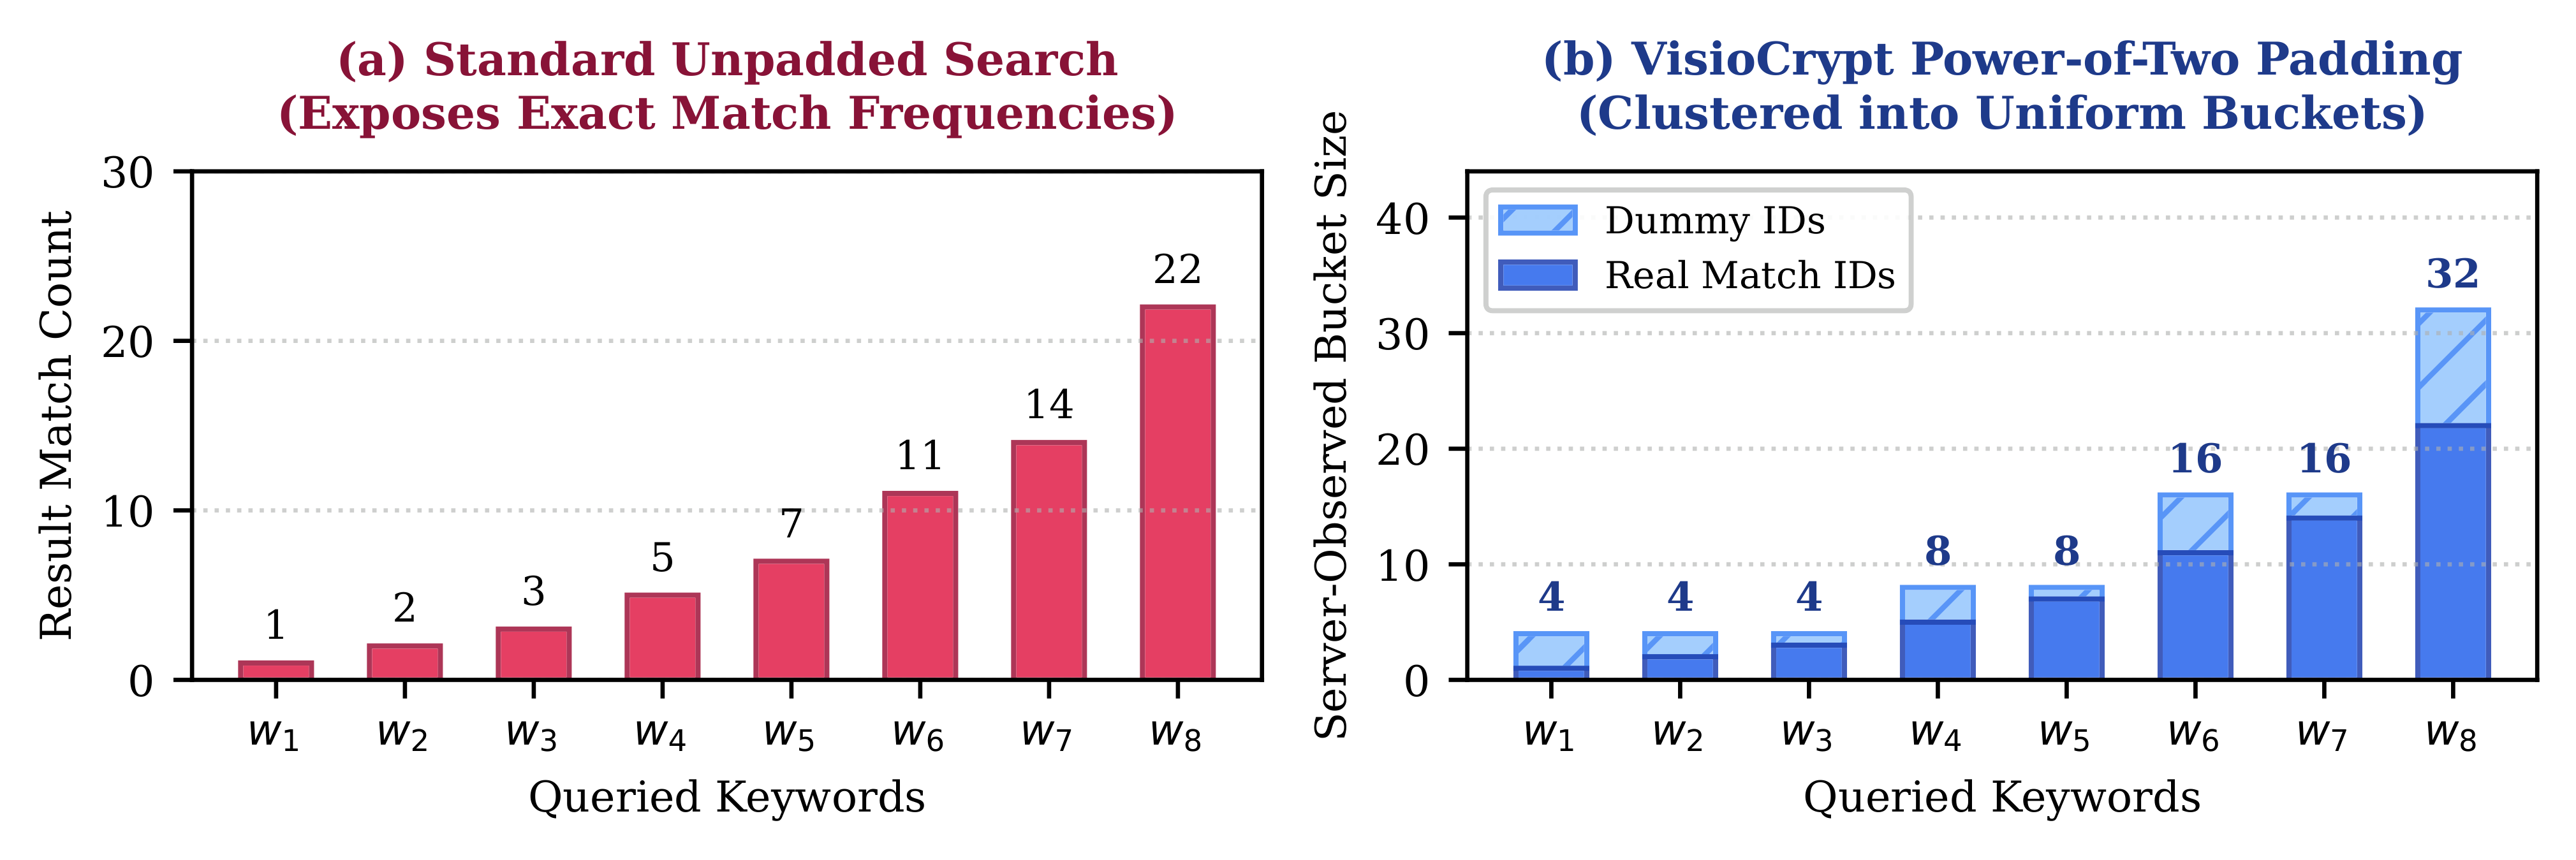
\includegraphics[width=\textwidth]{../writing_paper/figures/fig_volume_padding.png}
      \vspace{1mm}
      
      {\footnotesize Volume leakage vs. Power-of-Two Padding.}
    \end{column}
  \end{columns}
\end{frame}

% Slide 3: Architecture
\begin{frame}{VisioCrypt System Architecture}
  \begin{center}
    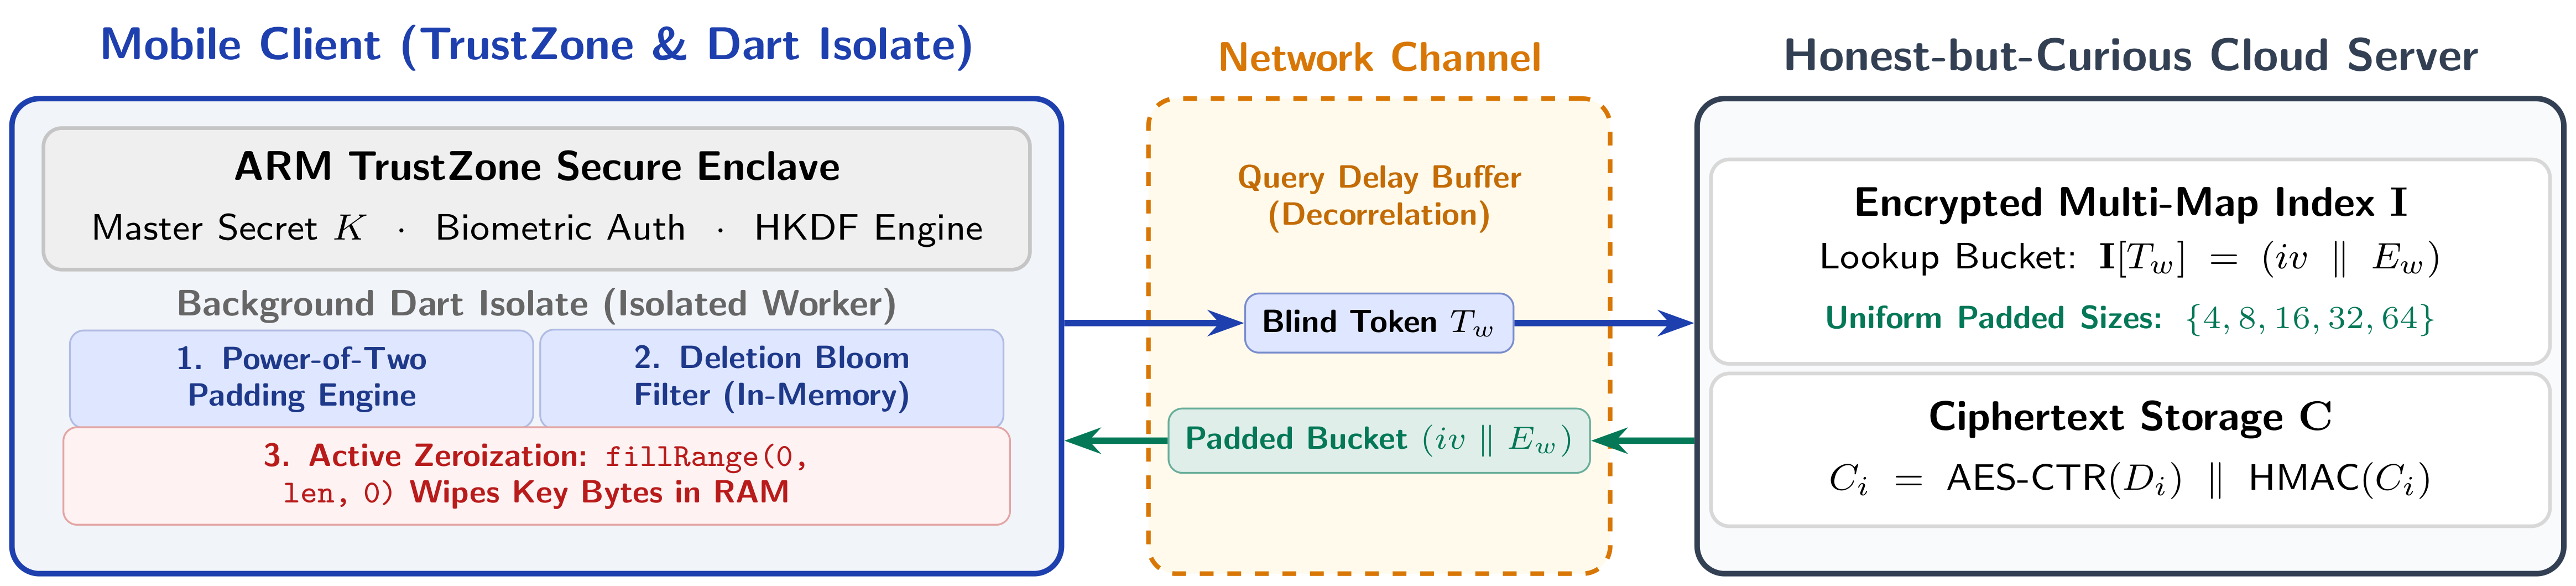
\includegraphics[width=0.88\textwidth]{../writing_paper/figures/fig_architecture.png}
  \end{center}
  \vspace{-2mm}
  \begin{itemize}
    \item \textbf{Mobile Client:} Master keys anchored in ARM TrustZone TEE; cryptography runs in Dart Isolates.
    \item \textbf{Network Channel:} Decorrelation delay buffer breaks temporal query correlations.
    \item \textbf{Cloud Server:} Blind index lookup ($\mathcal{O}(1)$) over encrypted multi-map; zero server-side plaintext access.
  \end{itemize}
\end{frame}

% Slide 4: Cryptographic Construction
\begin{frame}{Domain-Separated Cryptographic Construction}
  \begin{columns}
    \begin{column}{0.5\textwidth}
      \begin{block}{HKDF Master Key Derivation}
        From 256-bit hardware master key $K$:
        \begin{itemize}
          \item $K_{\text{enc}} \leftarrow \text{HKDF}(K, \text{``Doc-Enc''}, 32)$
          \item $K_{\text{search}} \leftarrow \text{HKDF}(K, \text{``Search-Trapdoor''}, 32)$
          \item $K_{\text{index}} \leftarrow \text{HKDF}(K, \text{``Index-Payload''}, 32)$
          \item $K_{\text{update}} \leftarrow \text{HKDF}(K, \text{``Delta-Update''}, 32)$
        \end{itemize}
      \end{block}
    \end{column}
    \begin{column}{0.5\textwidth}
      \begin{block}{Search \& Payload Primitives}
        \begin{itemize}
          \item \textbf{Trapdoor:} $T_w = \text{HMAC-SHA256}_{K_{\text{search}}}(w)$
          \item \textbf{Index Bucket:} $\mathbf{I}[T_w] = (iv \parallel \text{AES-GCM-Enc}_{K_{\text{index}}}(iv, L_w^*))$
          \item \textbf{File Ciphertext:} $C_i = \text{AES-CTR-256}_{K_{\text{enc}}}(D_i) \parallel \text{HMAC}(C_i)$
        \end{itemize}
      \end{block}
    \end{column}
  \end{columns}
\end{frame}

% Slide 5: Volume Hiding & Dynamic Bloom Filter
\begin{frame}{Volume Hiding and Dynamic Deletions}
  \begin{columns}
    \begin{column}{0.5\textwidth}
      \begin{block}{Power-of-Two Quantization ($\Phi$)}
        $$|\text{Pad}(L_w)| = \max\left(4, 2^{\lceil \log_2(|L_w|) \rceil}\right)$$
        \begin{itemize}
          \item Result sizes grouped into equivalence classes $\{4, 8, 16, 32, \dots\}$.
          \item Average storage inflation is only \textbf{$\approx 50.8\%$}.
        \end{itemize}
      \end{block}
    \end{column}
    \begin{column}{0.5\textwidth}
      \begin{block}{Dynamic Deletions via Local Bloom Filter}
        $$m = -\frac{n \ln p}{(\ln 2)^2} \approx 117\text{ KB}, \quad k = \frac{m}{n}\ln 2 \approx 13$$
        \begin{itemize}
          \item Tracks 50,000 deletions locally ($P_e \le 10^{-4}$).
          \item Type-II Backward Privacy achieved in \textbf{$< 0.08\text{ ms}$} without cloud notification.
        \end{itemize}
      \end{block}
    \end{column}
  \end{columns}
\end{frame}

% Slide 6: Mobile Memory Hygiene
\begin{frame}{Mobile Memory Hygiene and Heap Protection}
  \begin{columns}
    \begin{column}{0.5\textwidth}
      \begin{alertblock}{The Android Heap Scraping Threat}
        Standard garbage collectors (ART VM) allow sensitive keys to linger in volatile RAM for minutes after use, vulnerable to memory inspection.
      \end{alertblock}
      \begin{block}{VisioCrypt Memory Defense}
        \begin{itemize}
          \item Isolated execution via \textbf{Dart Isolates}.
          \item Keys stored exclusively as contiguous \texttt{Uint8List} buffers.
          \item Explicit \textbf{active zeroization} (\texttt{fillRange(0, len, 0)}) runs immediately ($< 1\text{ ms}$) after cipher calls.
        \end{itemize}
      \end{block}
    \end{column}
    \begin{column}{0.48\textwidth}
      \centering
      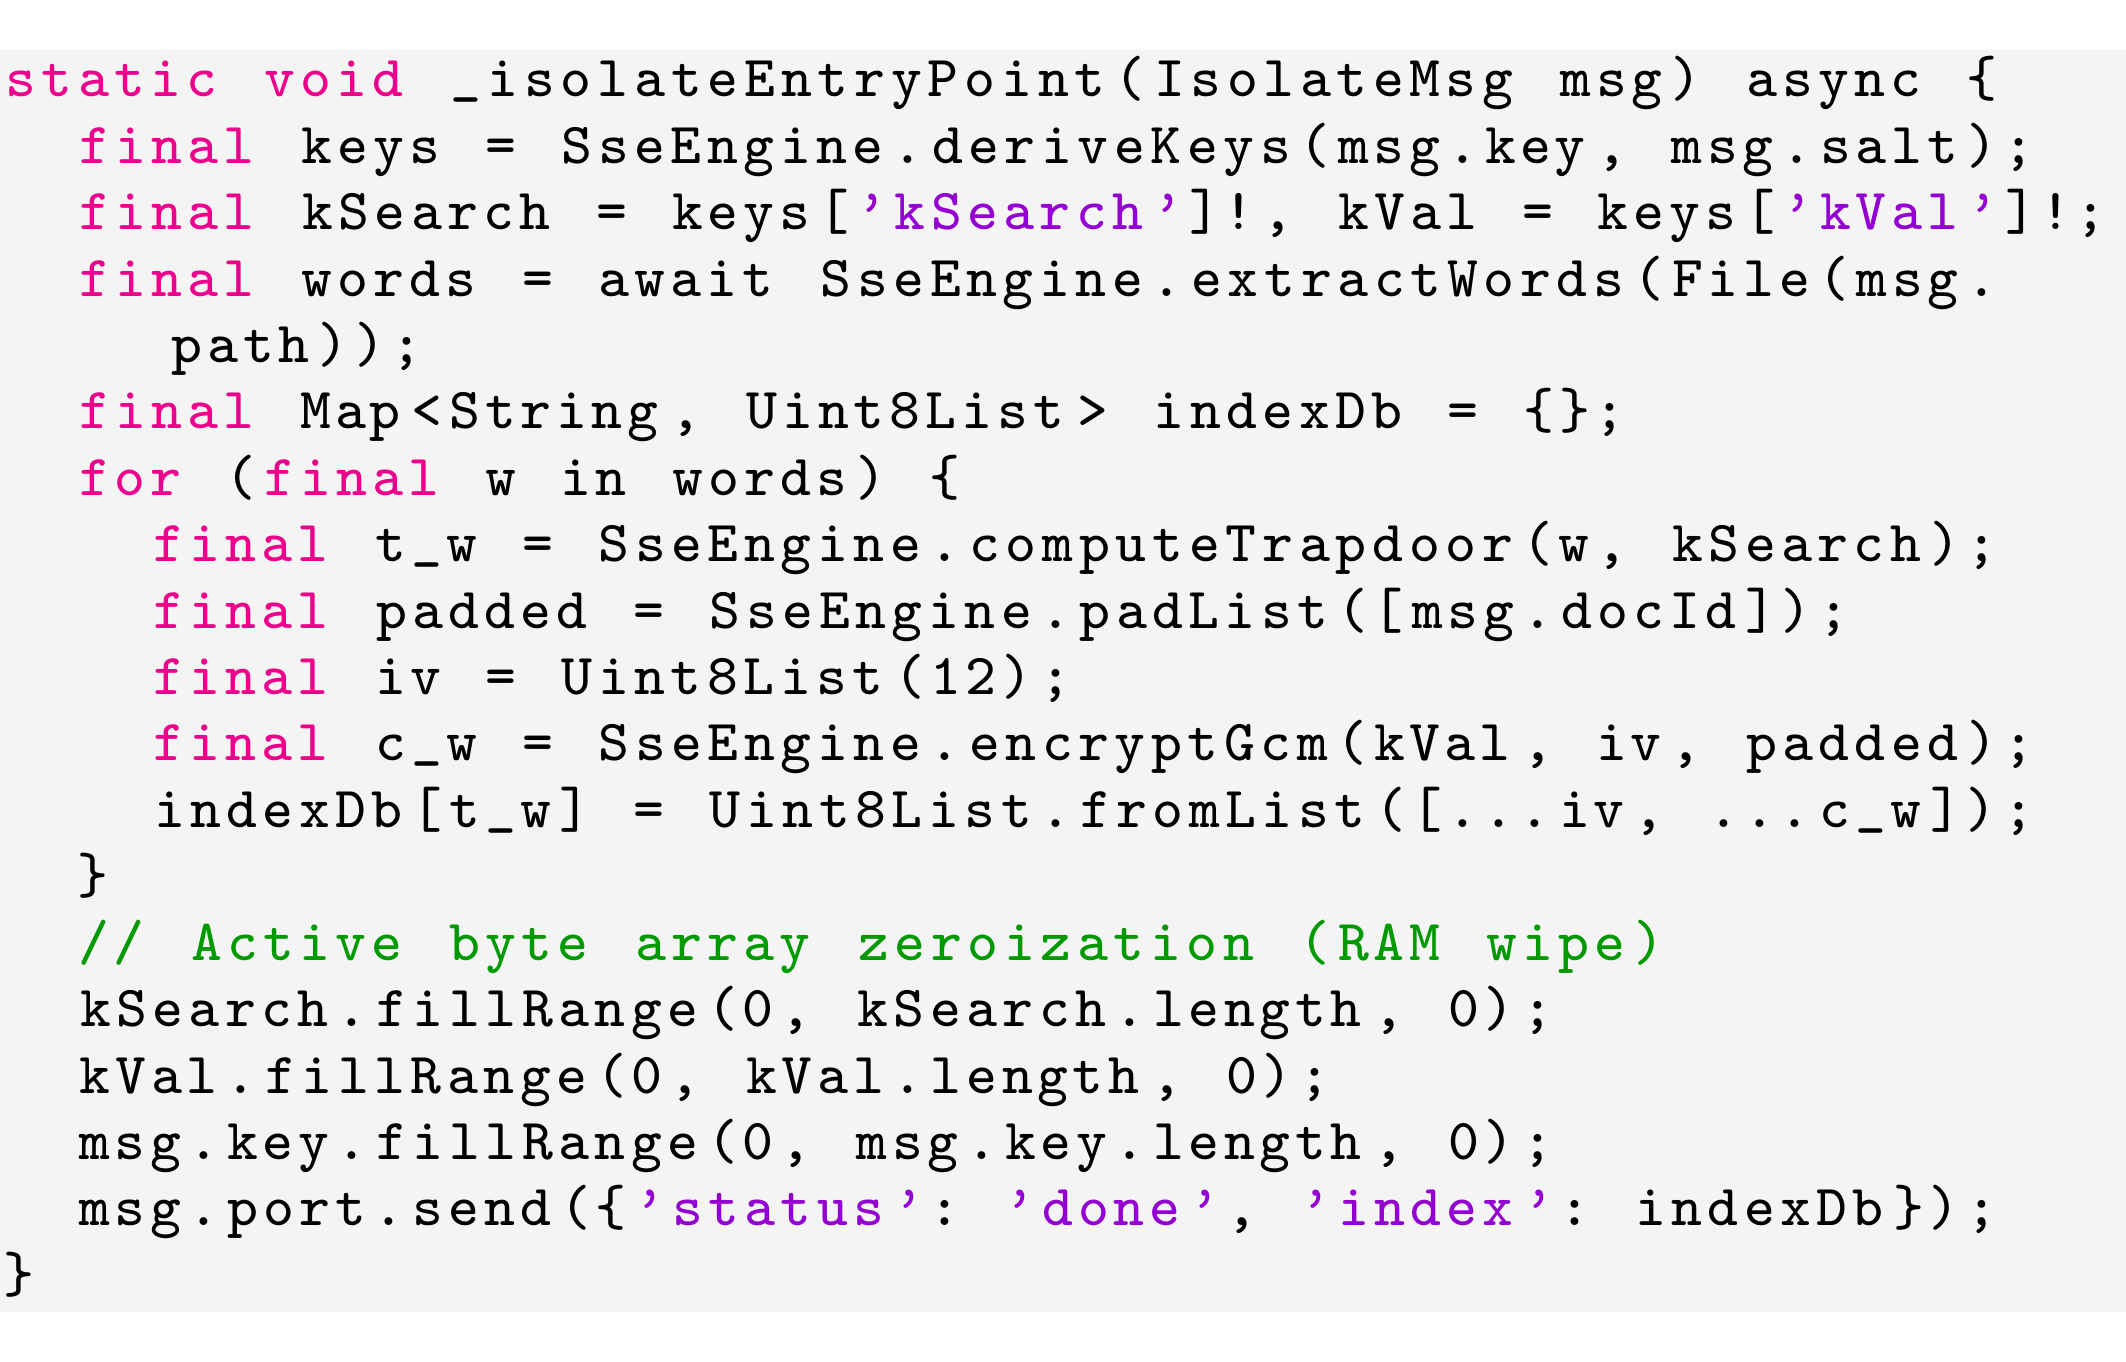
\includegraphics[width=\textwidth]{../writing_paper/figures/lst_isolate.png}
    \end{column}
  \end{columns}
\end{frame}

% Slide 7: Hardware Testbed & Encryption Throughput
\begin{frame}{Empirical Hardware Testbed \& File Throughput}
  \begin{columns}
    \begin{column}{0.48\textwidth}
      \centering
      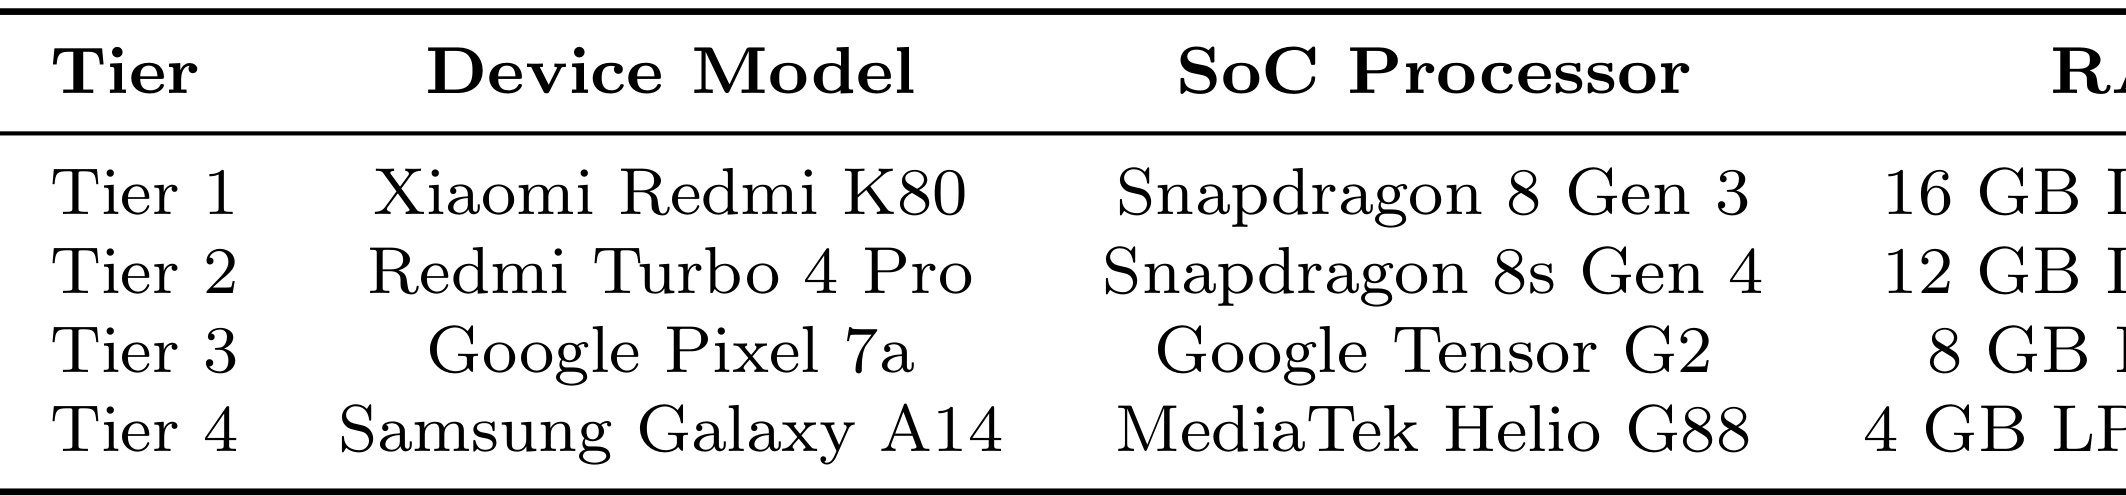
\includegraphics[width=\textwidth]{../writing_paper/figures/tab_testbed.png}
      \vspace{2mm}
      \footnotesize Four diverse mobile tiers tested (Snapdragon 8 Gen 3 to MediaTek Helio G88).
    \end{column}
    \begin{column}{0.48\textwidth}
      \centering
      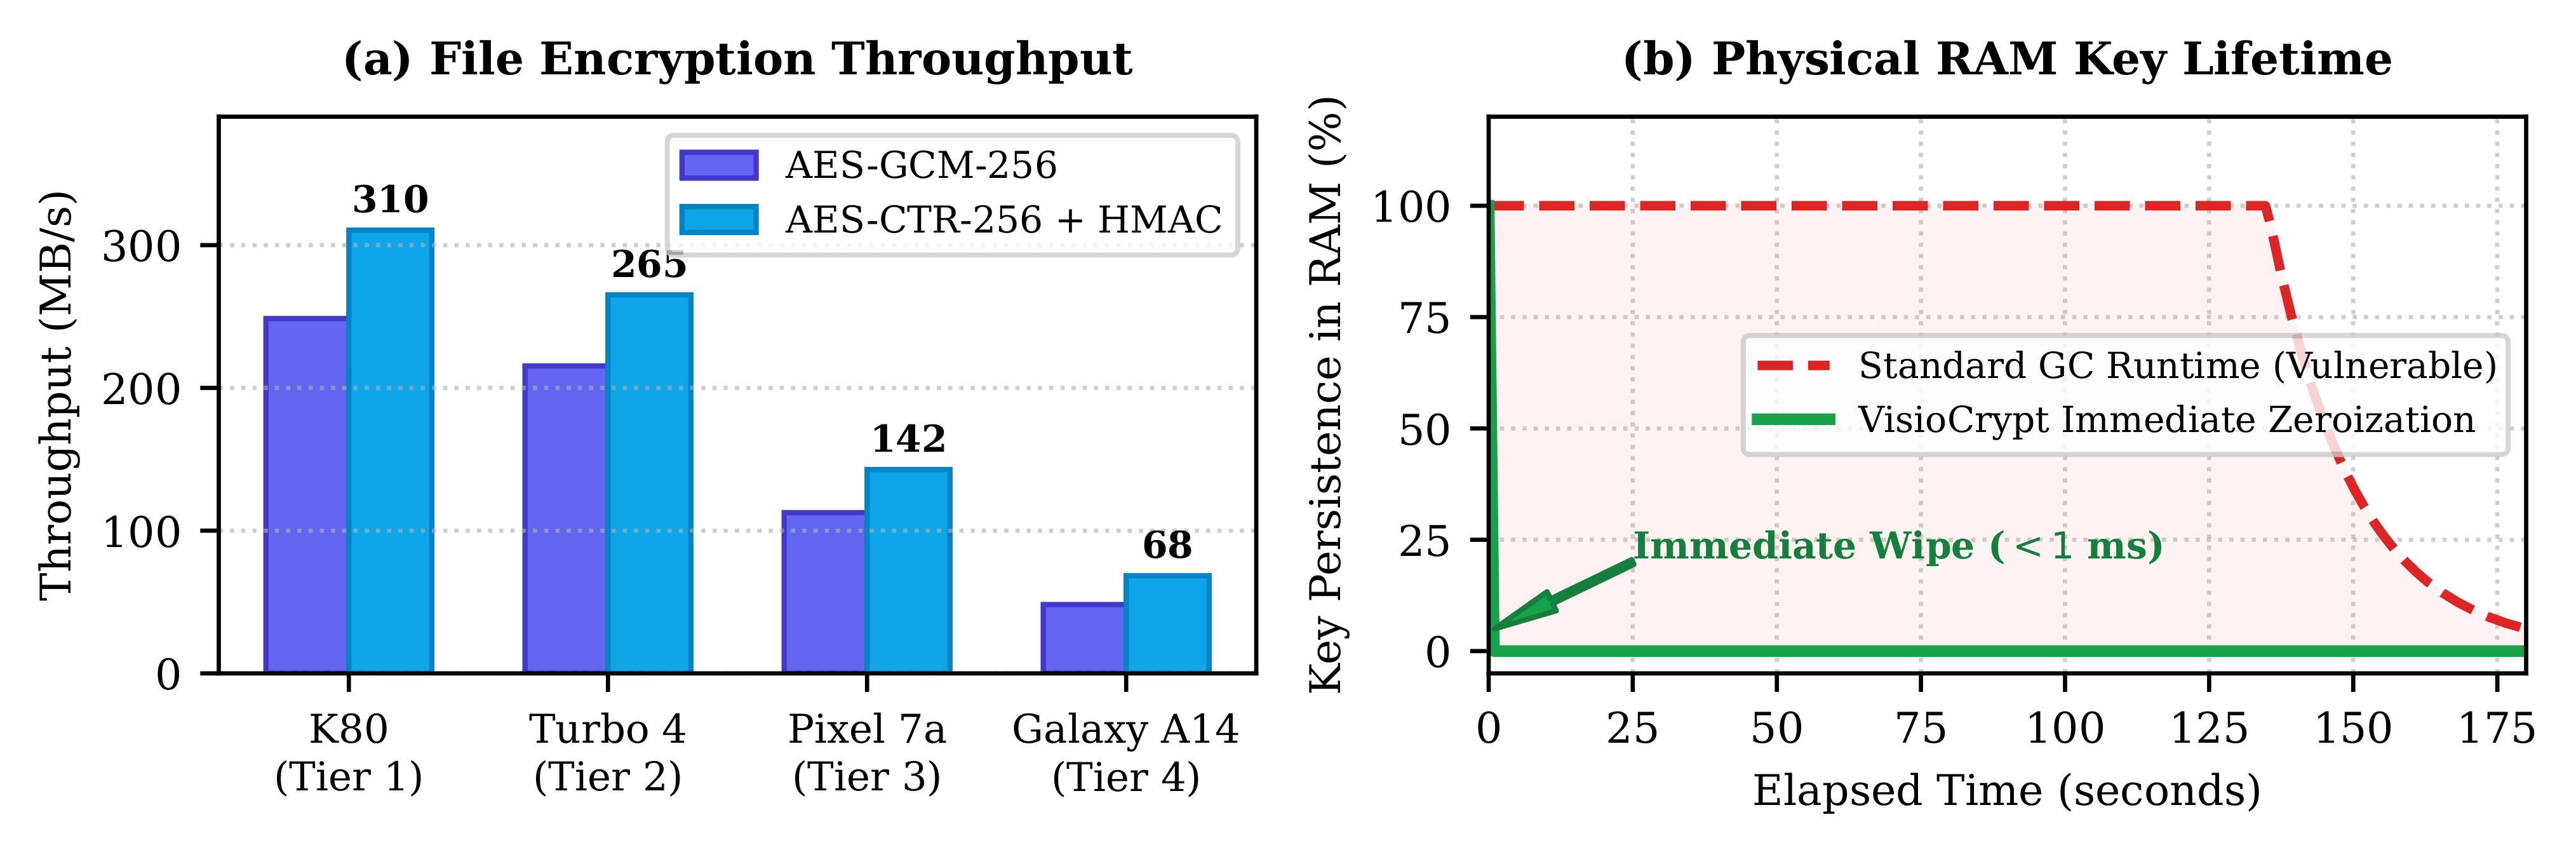
\includegraphics[width=\textwidth]{../writing_paper/figures/fig_throughput_benchmark.png}
      \vspace{1mm}
      \footnotesize Peak encryption throughput reaches \textbf{310.5 MB/s} on Redmi K80.
    \end{column}
  \end{columns}
\end{frame}

% Slide 8: Search Query Latency
\begin{frame}{Search Latency Across Smartphone Tiers}
  \begin{center}
    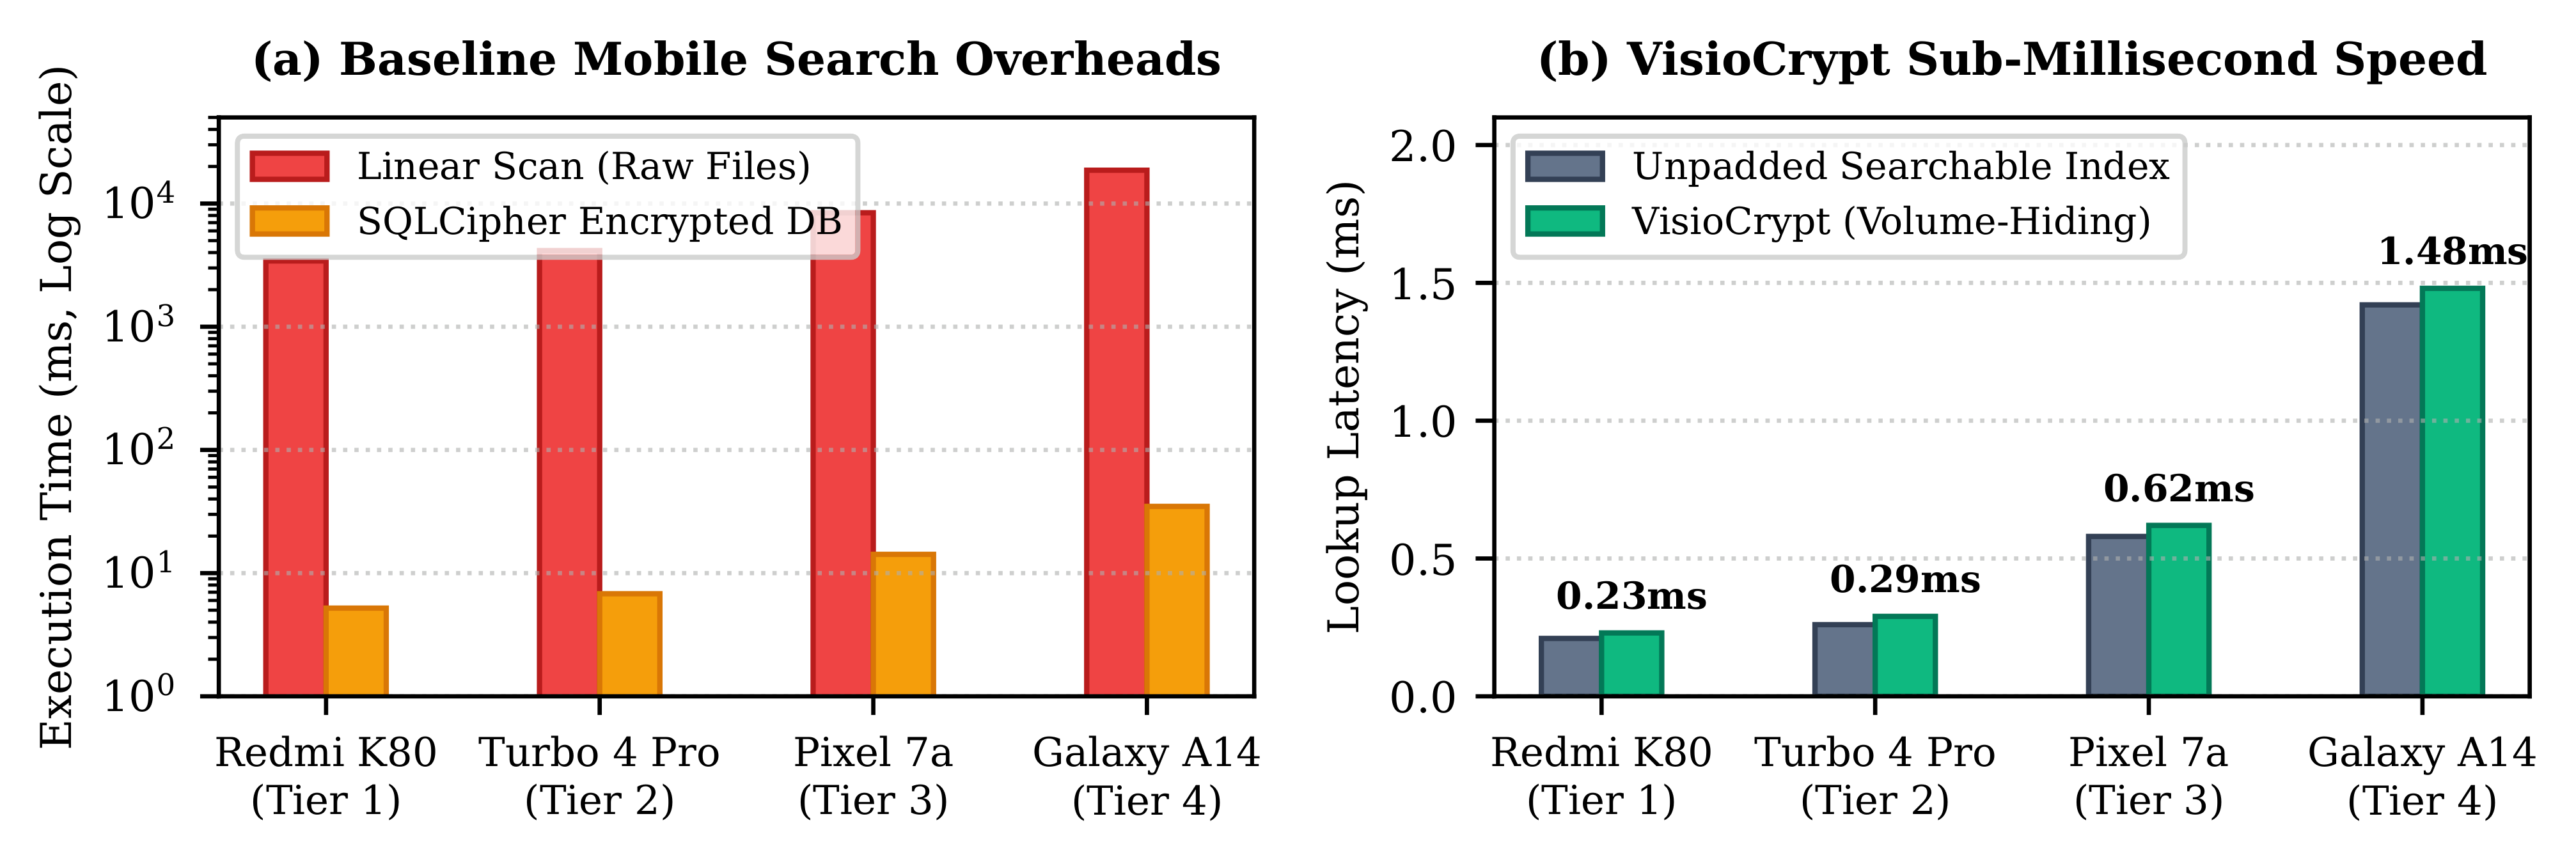
\includegraphics[width=0.85\textwidth]{../writing_paper/figures/fig_search_latency.png}
  \end{center}
  \vspace{-2mm}
  \begin{itemize}
    \item \textbf{Sub-Millisecond Search:} $0.23\text{ ms}$ on Redmi K80, $0.29\text{ ms}$ on Turbo 4, $0.62\text{ ms}$ on Pixel 7a.
    \item \textbf{Budget Device Efficiency:} $1.48\text{ ms}$ on Galaxy A14 ($12,600\times$ faster than linear scan).
    \item \textbf{Negligible Volume-Hiding Cost:} Adding padding overhead adds only $+0.02\text{ ms}$ to $+0.06\text{ ms}$ latency.
  \end{itemize}
\end{frame}

% Slide 9: State-of-the-Art Comparison
\begin{frame}{State-of-the-Art Comparison}
  \resizebox{\textwidth}{!}{%
  \begin{tabular}{lcccccc}
    \toprule
    \textbf{Scheme} & \textbf{Year} & \textbf{Complexity} & \textbf{Dynamic} & \textbf{Volume Hiding} & \textbf{Forward Priv.} & \textbf{Backward Priv.} \\
    \midrule
    Song et al. & 2000 & $\mathcal{O}(N)$ Linear & No & No & No & No \\
    Curtmola et al. & 2006 & $\mathcal{O}(|L_w|)$ Sub-linear & Static & No & No & No \\
    SEAL (Demertzis et al.) & 2020 & $\mathcal{O}(|L_w|)$ Sub-linear & Yes & Batch ($x$) & Yes & Type-II \\
    SWAT (Ihsan et al.) & 2024 & $\mathcal{O}(|L_w|)$ Sub-linear & Yes & Bucket Partition & Heuristic & No \\
    SGX-SE2 (Liu et al.) & 2021 & $\mathcal{O}(|L_w|)$ Sub-linear & Yes & No & Yes & Type-II (Server SGX) \\
    \midrule
    \textbf{VisioCrypt (Ours)} & \textbf{2026} & $\boldsymbol{\mathcal{O}(|L_w|)}$ \textbf{Sub-linear} & \textbf{Yes} & \textbf{Power-of-Two ($\Phi$)} & \textbf{Yes} & \textbf{Type-II (Client BF)} \\
    \bottomrule
  \end{tabular}%
  }
  \vspace{2mm}
  \begin{block}{Why VisioCrypt Stands Out}
    \begin{itemize}
      \item \textbf{No Cloud Hardware Enclaves Required:} Works over standard cloud storage (S3, Drive).
      \item \textbf{Complete Forward \& Backward Privacy:} Local Bloom filtering achieves Type-II BP without ORAM.
      \item \textbf{Hardware-Anchored Mobile Hygiene:} Combines TrustZone keys with active RAM zeroization.
    \end{itemize}
  \end{block}
\end{frame}

% Slide 10: Conclusion & Summary
\begin{frame}{Summary and Key Takeaways for Faculty Evaluation}
  \begin{columns}
    \begin{column}{0.5\textwidth}
      \begin{block}{Scientific Novelties}
        \begin{enumerate}
          \item First client-side volume-hiding SSE tailored for commodity mobile handsets.
          \item Sub-millisecond dynamic deletions via local Bloom filtering ($117\text{ KB}$).
          \item Active Dart isolate memory zeroization bounding key exposure to $< 1\text{ ms}$.
        \end{enumerate}
      \end{block}
    \end{column}
    \begin{column}{0.5\textwidth}
      \begin{block}{Practical Impact}
        \begin{itemize}
          \item \textbf{Ultra-Fast Retrieval:} $0.23 - 1.48\text{ ms}$ search across 10,000 keywords.
          \item \textbf{Negligible Energy:} 1,000 searches consume only $1.85\text{ mJ}$.
          \item \textbf{Zero Cloud Modification:} Works out-of-the-box with AWS S3, Google Drive, and Dropbox.
        \end{itemize}
      \end{block}
    \end{column}
  \end{columns}
  \vspace{3mm}
  \centering
  \textbf{\large Thank You! Questions \& Discussion}
\end{frame}

\end{document}
